% Created 2020-10-25 So 23:03
% Intended LaTeX compiler: pdflatex
\UseRawInputEncoding

\documentclass[11pt]{scrartcl}
\usepackage[utf8]{inputenc}
\usepackage[T1]{fontenc}
\usepackage[ngerman]{babel}
\usepackage{graphicx}
\usepackage{grffile}
\usepackage{longtable}
\usepackage{wrapfig}
\usepackage{rotating}
\usepackage[normalem]{ulem}
\usepackage{amsmath}
\usepackage{upgreek}
\usepackage{trfsigns}
\usepackage{textcomp}
\usepackage{amssymb}
\usepackage{capt-of}
\usepackage{MnSymbol}
\usepackage{mathtools}
\usepackage{setspace}
\usepackage{nicematrix}
\usepackage{empheq}
\usepackage{pdfpages}
% \usepackage{getlab}
\usepackage{listings}
\usepackage{pdfpages}
\usepackage[straightvoltages, european resistors, european inductors]{circuitikz}
\usetikzlibrary{arrows.meta}
\tikzset{FARROW/.style={arrows={-Triangle[angle=45:2.0mm]}}}
% \usepackage{varwidth}
\usepackage{hyperref}


\definecolor{darkspringgreen}{rgb}{0.09, 0.45, 0.27}    % Farbe für die Kommentare bei Listings
% \lstset{
%   language= Matlab,                     % Setzt die Sprache
%   basicstyle=\scriptsize\ttfamily,     % Setzt den Standardstil
%   % keywordstyle=\color{red}\bfseries,    % Setzt den Stil für Schlüsselwörter
%   identifierstyle=\color{blue},        % Identifier bekommen keine gesonderte formatierung
%   commentstyle=\color{darkspringgreen},        % Stil für Kommentare
%   stringstyle=\ttfamily,             % Stil für Strings (gekennzeichnet mit "String")
%   breaklines=true,             % Zeilen werden umgebrochen
%   numbers=left,                 % Zeilennummern links
%   numberstyle=\tiny,             % Stil für die Seitennummern
%   frame=single,                 % Rahmen
%   % backgroundcolor=\color{myGrey},     % Hintergrundfarbe
%   % caption={Java-Code},             % Caption
%   tabsize=2                % Größe der Tabulatoren
% }



\newcommand{\GETHeader}[6]{%
  \begin{titlepage}
    \pagestyle{empty} \enlargethispage*{25cm}\samepage{
      \vspace*{-2.5cm}
      \begin{center}
        %
        \begin{tabular}[b]{lr}
          %
          \hspace*{-1.5cm}
          \begin{tabular}{p{3.8cm}}
            
\includegraphics[width=3.8cm]{./Figures/TUGraz}
          \end{tabular}
          %
          \hspace*{-1cm}
          %
          %
          \begin{tabular}{p{13.8cm}}
            \begin{flushright}
              \large
              Institut für Grundlagen und Theorie der Elektrotechnik\\
              ~\\
            \end{flushright}
          \end{tabular}
        \end{tabular}

        \vspace*{2.2cm}
        %
        \Huge {Elektrische Netzwerke und Mehrtore \\ Übung\\} %
        \vspace*{.5cm} \Large{ Wintersemester 2020\\}
        %
        \vspace*{1.5cm}

        \Huge{\textbf{#1}\\}

        %
        % \vspace*{0.8cm} \Large{Übungsdatum: {#2}\\}
        %
        \vspace*{1cm} \vfill
        %
        \Large{Gruppe: {#2}\\} \vspace*{0.5cm}%


        % \Large{Protokollführer(in): {#3}\\} \vspace*{1cm}

        \Large{Gruppenteilnehmer:\\} \vspace*{.1cm}
        % Name der beteiligten Studierenden
        \Large{#3} \vspace{1cm}
        %
        %
        \Large{Vortragende: #4\\} \vspace*{.1cm}   %\vspace*{1.5cm}
        % \Large{Betreuer(in): #6\\}
        \vspace*{1.5cm}
        %
        \Large{#5, am #6}
      \end{center}}%
    %
    \clearpage
  \end{titlepage}}


\definecolor{codegreen}{rgb}{0,0.6,0}
\definecolor{codegray}{rgb}{0.5,0.5,0.5}
\definecolor{codepurple}{rgb}{0.58,0,0.82}
\definecolor{backcolour}{rgb}{0.95,0.95,0.92}

\lstdefinestyle{mystyle}{
    backgroundcolor=\color{backcolour},
    commentstyle=\color{codegreen},
    keywordstyle=\color{magenta},
    numberstyle=\tiny\color{codegray},
    stringstyle=\color{codepurple},
    basicstyle=\ttfamily\footnotesize,
    breakatwhitespace=false,
    breaklines=true,
    captionpos=b,
    keepspaces=true,
    numbers=left,
    numbersep=5pt,
    showspaces=false,
    showstringspaces=false,
    showtabs=false,
    tabsize=2
}

\lstset{style=mystyle}







\begin{document}

\GETHeader                                                                              %  Bitte Ausfüllen!!!
% ----------------------------
{Protokoll Übung 6: \\ Fourieranalyse}                         %  Übungstitel
% ----------------------------
% {25. Mai 2020}                                                                  %  Übungsdatum
% ----------------------------
{04}                                                                   %  Gruppen-Nr.
% ----------------------------
% {Matthias Fottner}                                                                      % Name des Protokollführers oder der Protokollführerin
% ----------------------------
{
  \begin{center}
    \begin{minipage}{0.28\linewidth}
      1. Matthias Fottner\\
      2. David Keller\\
      3. Moritz Woltron
    \end{minipage}
  \end{center}
}
% ----------------------------
{Helena Grabner}                                                                     %  Laborleiter(in)
% {Übung 2}                                                               %  Betreuer(in)
% ----------------------------
{Graz}                                                                                  %  Ort der Protokollerstellung
{\today}`                                                                %  Datum Protokollerstellung


\newcommand{\unit}[1]{\,\text{#1}}


\tableofcontents

\newpage


\allowdisplaybreaks

\setlength{\jot}{10pt}

\section{Numerische Bestimmung der Fourierreihenkoeffizienten von $u_{in}(t)$}
Die Fourierreihe einer Funktion lässt sich folgendermaßen notieren:
\begin{align*}
  a_{0} + \sum\limits_{k=1}^{\infty} \left[ a_{k} \cos(k\omega_{0}t) + b_{k} \sin(k \omega_{0}t)\right]
\end{align*}
Da es keinen Gleichanteil gibt, ist $a_{0}=0$.
Aufgrund der ungeraden Symmetrie sind alle Koeffizienten $a_{k} = 0$.
Die Koeffizienten $b_{k}$ werden in Matlab numerisch mit der Trapezmethode angenähert.
Mit der Funktion \lstinline{b_k} (Kapitel \ref{sec:plot_1}, Z. 50-56 ) erhält man für die ersten Koeffiziente:

\begin{figure}[!htb]
  \centering
\begin{lstlisting}[language=Python]
  b_1 = 41.64106231
  b_2 = -4.87735577
  b_3 = 2.25902828
  b_4 = -3.78545704
  b_5 = 2.54658425
\end{lstlisting}
\caption{Die Grundschwingung $b_1$ und die ersten 4 Oberschwingungen $b_{2-5}$}
\end{figure}
\newpage
\section{Plot der ersten 5 Schwingungen}
\begin{figure}[!htb]
    \begin{center}
    % \hspace{3cm}
      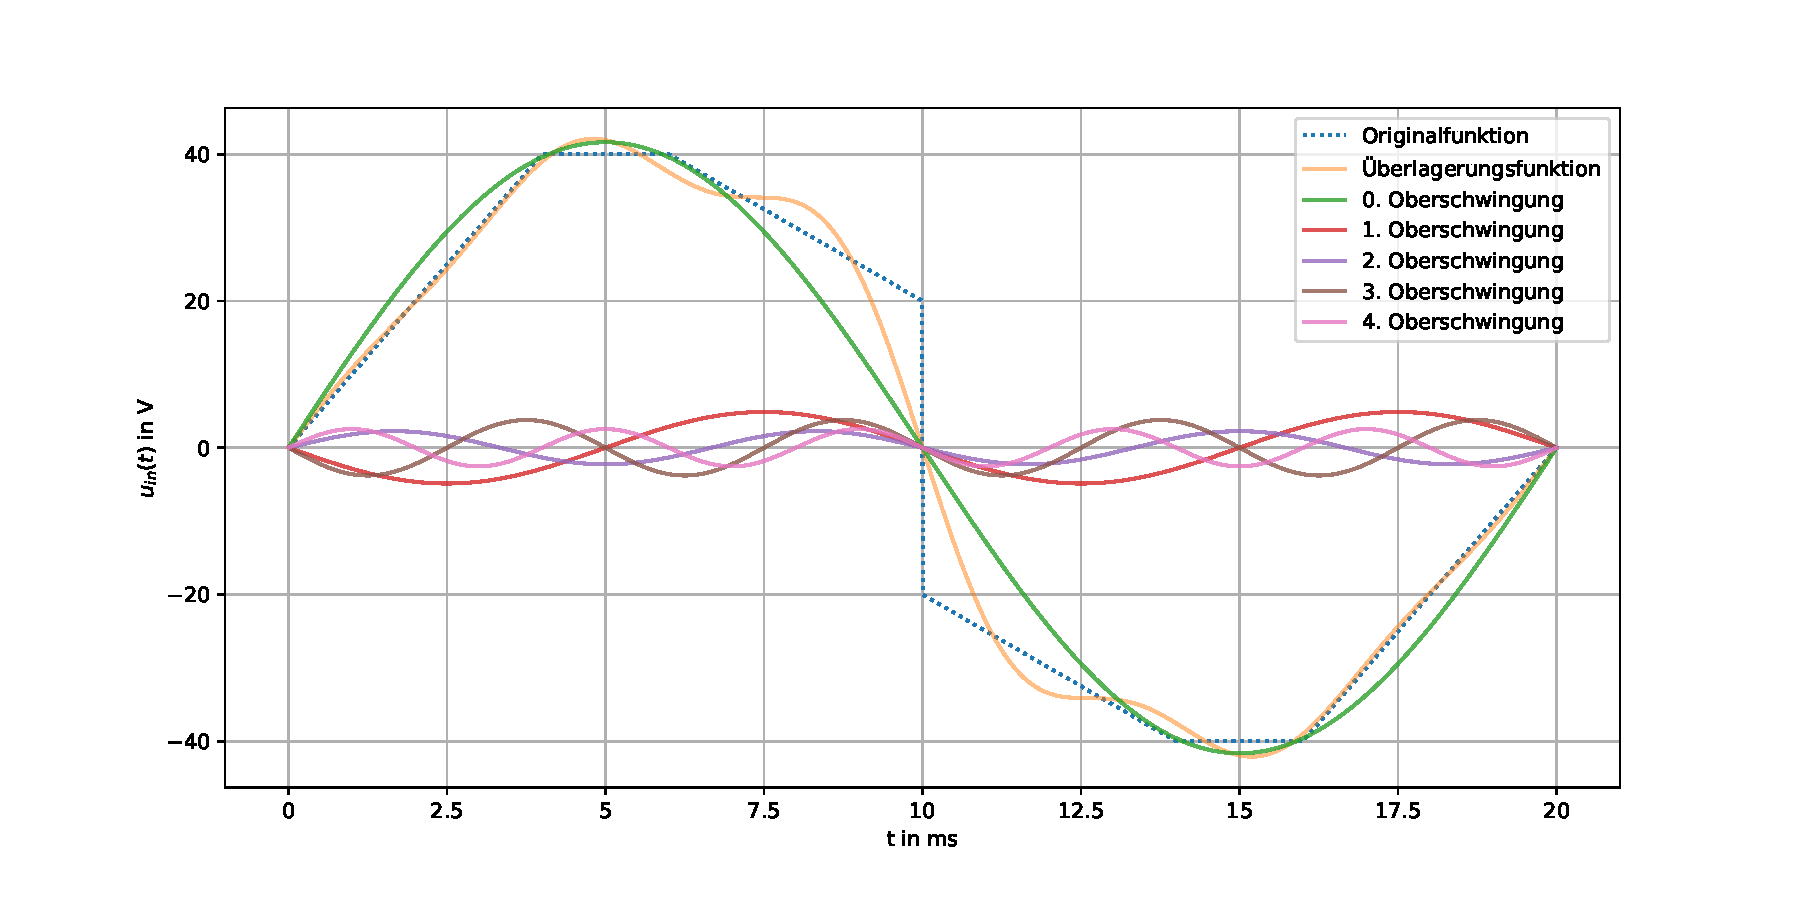
\includegraphics[width=1.1\linewidth]{./Figures/plot_1.pdf}
    \caption{Plot der Grundschwingung und der ersten 4 Oberschwingungen, sowie deren Überlagerung}
    \label{fig:plot_1}
  \end{center}
\end{figure}
\newpage
\section{Plot der ersten 250 Wellen}
\begin{figure}[!htb]
    \begin{center}
      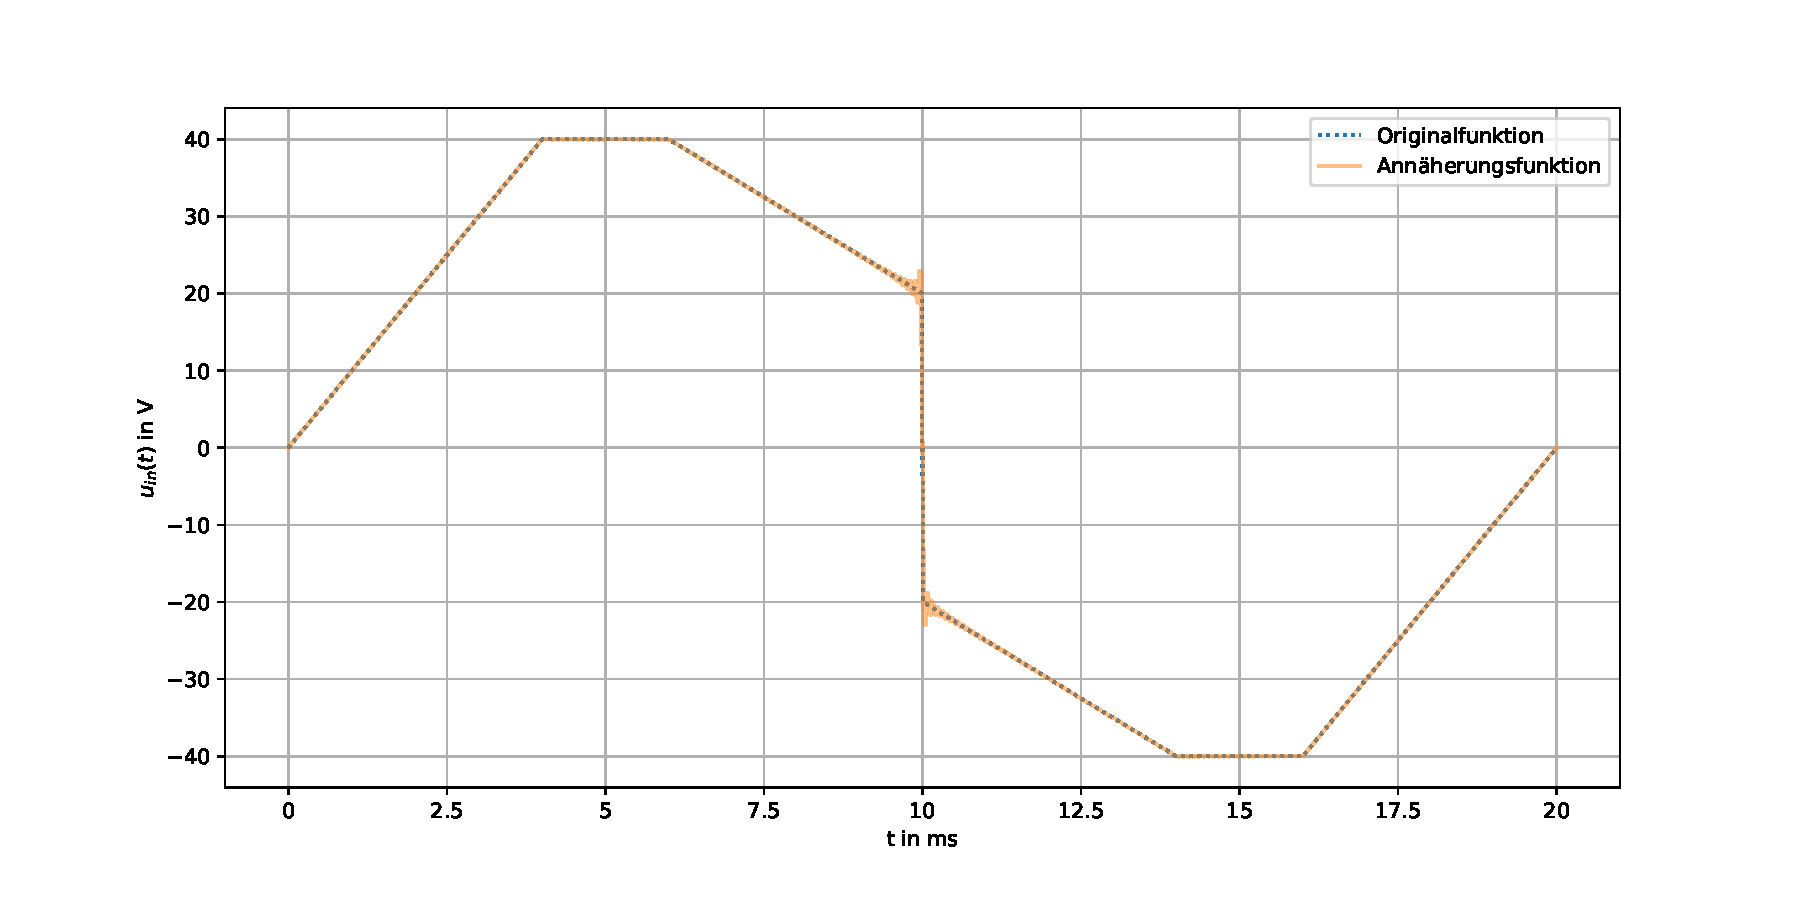
\includegraphics[width=1.1\linewidth]{./Figures/plot_2.pdf}
    \caption{Plot der Fourierreihe mit den ersten 250 Wellen}
    \label{fig:plot_2}
  \end{center}
\end{figure}
Wie in Abbildung \ref{fig:plot_2} ersichtlich, strebt die Fourierreihe(orange) gegen die Originalfunktion(blau). Da bei $t=\frac{T}{2}$ eine Sprungstelle existiert, nimmt die Fourierreihe dort den Mittelwert der Sprungstelle an. In diesem Fall ist das 0.
Somit ist $u_{in}(t=\frac{T}{2}) = 0$.

\section{Bestimmen der Induktivität $L$}
Um die Induktivität der Spule zu bestimmen, ist es sinnvoll zuerst die Übertragungsfunktion $H(j\omega)$ zu bestimmen:
\begin{align*}
  \underline{H}(j\omega) &= \frac{\underline{U}_{out}}{\underline{U}_{in}} \\
                         &= \frac{R}{R + j\omega L} \\
                         &= \frac{1}{1 + \frac{j\omega}{\frac{R}{L}}} \\
                        \Longrightarrow \Omega &= \frac{R}{L}
\end{align*}
Die dritte Oberschwingung $\omega_{3}$ soll bereits um $-3 \unit{dB}$ verstärkt werden. Das ist der Fall, wenn $\omega_{3} \overset{!}{=} \Omega$ gilt.
\begin{align*}
  \Omega &= \omega_{3} = 4\cdot\omega_{0} = 4\cdot\frac{2 \pi}{T} = 400 \pi\ \frac{1}{\text{s}} \\
  \Omega &= \frac{R}{L} \\
  L &= \frac{R}{\Omega} = \frac{2\pi \unit{$\Omega$}}{400 \pi\ \frac{1}{\text{s}}} \\
         &= 6,67 \unit{mH}
\end{align*}
\newpage
\section{Bestimmen des Ausgangssignals $u_{out}(t)$}
Jede Oberschwingung $u_{in,k}$ wird mit dem Betrag der Übertragungsfunktion multipliziert, weiterhin wird der Winkel im Argument addiert. Es ergibt sich:
\begin{align*}
  u_{out,k} &= b_{k} \cdot |H(j\omega)|\cdot \cos(k\omega_{0}t + arg(H(j\omega)))
\end{align*}
$u_{out}$ ergibt sich aus der Summe der Schwingungen $u_{out,k}$:
\begin{align*}
  u_{out} &= \sum\limits_{k=1}^{\infty} u_{out,k}
\end{align*}

Dies wurde in der Funktion \lstinline{u_out()} (Kapitel \ref{sec:plot_3}, ab Z. 78) implementiert und in Abbildung \ref{fig:plot_3} geplottet.
\begin{figure}[!htb]
    \begin{center}
    % \hspace{3cm}
      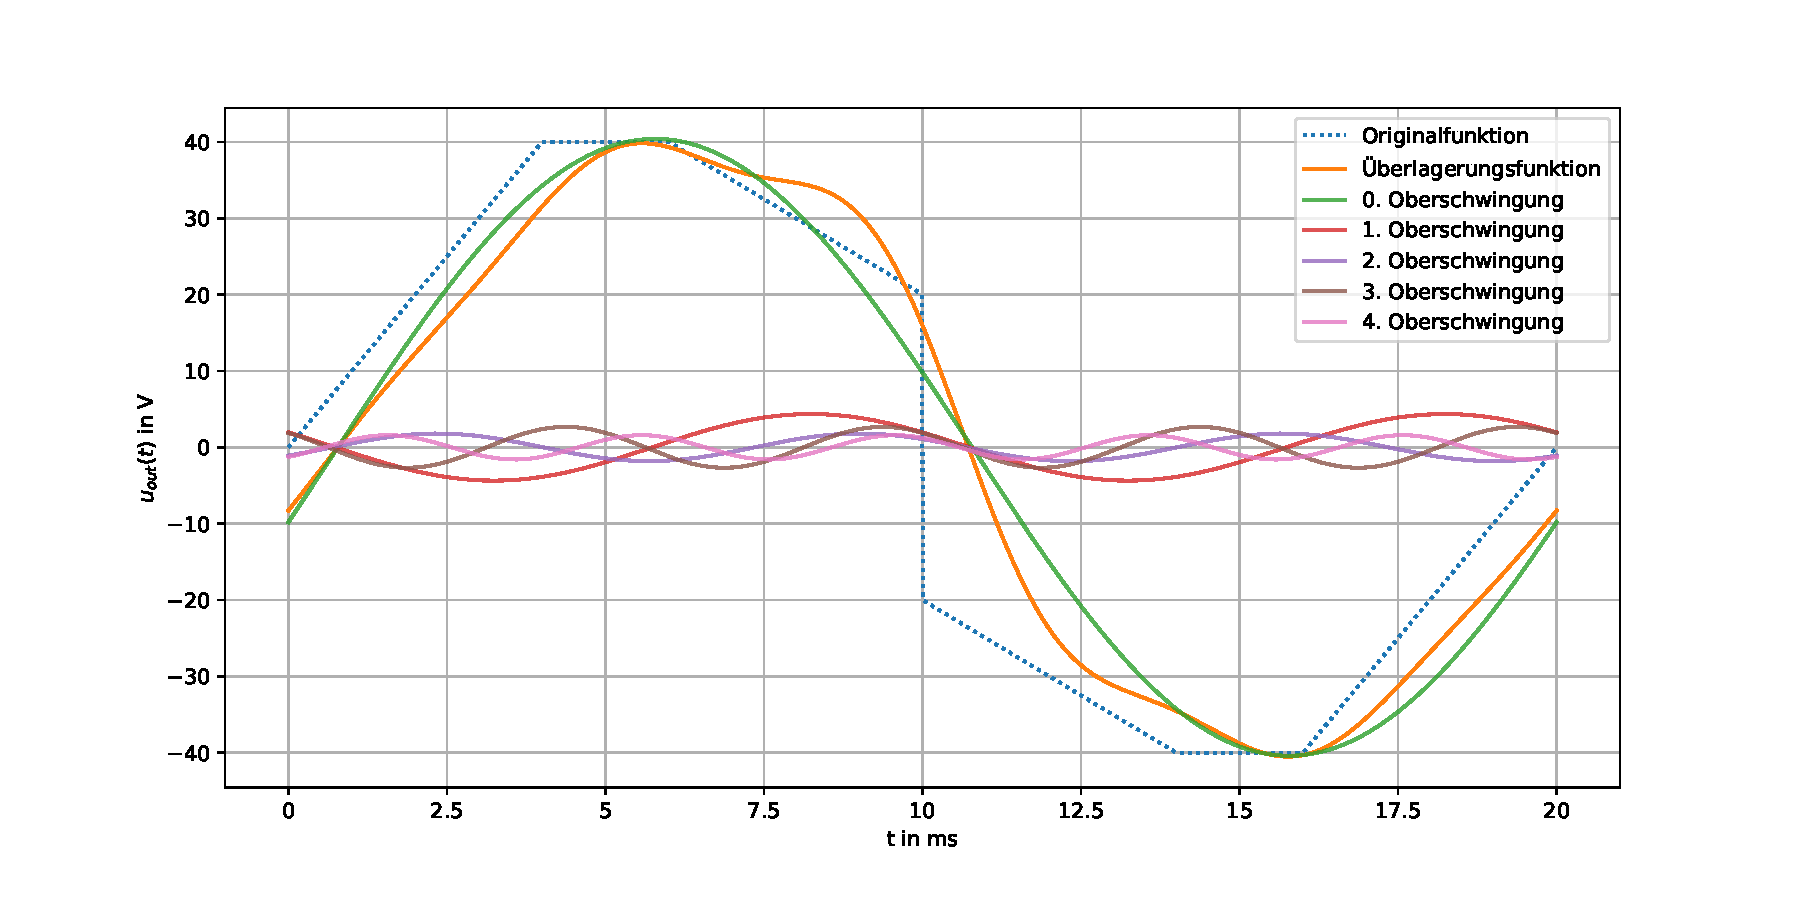
\includegraphics[width=1.1\linewidth]{./Figures/plot_3.pdf}
    \caption{Plot Ausgangsspannung $u_{out}(t)$ und dessen Oberschwingungen}
    \label{fig:plot_3}
  \end{center}
\end{figure}

Betrag und Phasenwinkel wurden in Funktion \lstinline{u_out()} (Kapitel \ref{sec:plot_3}, Z. 89) als print ausgegeben und anschließend in Abbildung \ref{fig:bet-phas} aufgelistet. Es fällt auf, dass der Betrag der Wellen mit steigendem $\omega$ abnimmt. Deshalb handelt es sich auch wirklich um einen Tiefpass-Filter.
Weiterhin fällt der Phasenwinkel von $-45^{\circ}$ bei der 3. Oberschwingung auf. Da diese Oberschwingung eine Verstärkung von $-3 \unit{dB}$ haben sollte, dient diese als Grenzfrequenz.
Die Grenzfrequenz hat die Eigenschaft, einen Phasenwinkel von $45^{\circ}$ zu besitzen. Dadurch bestätigen sich die Berechnungen.
\begin{figure}[!htb]
  \centering
\begin{lstlisting}[language=Python]
0. Oberschwingung: |H(jw)|: 0.9701,      arg(H(jw)): -14.0362°
1. Oberschwingung: |H(jw)|: 0.8944,      arg(H(jw)): -26.5651°
2. Oberschwingung: |H(jw)|: 0.8,         arg(H(jw)): -36.8699°
3. Oberschwingung: |H(jw)|: 0.7071,      arg(H(jw)): -45.0°
4. Oberschwingung: |H(jw)|: 0.6247,      arg(H(jw)): -51.3402°
\end{lstlisting}
\caption{Betrag und Phasenwinkel der ersten 5 Oberschwingungen}
\label{fig:bet-phas}
\end{figure}

\section{Python-Skripte}
\subsection{plot\_1.py}\label{sec:plot_1}
\lstinputlisting[language=Python]{./plot_1.py}
\subsection{plot\_2.py}
\lstinputlisting[language=Python]{./plot_2.py}
\subsection{plot\_3.py}\label{sec:plot_3}
\lstinputlisting[language=Python]{./plot_3.py}
\end{document}
